% В этом файле вы описываете задачи из контеста
% Условия можно вставить в виде фотографий
% В идеях нужно написать хотя бы два-три предложения о задаче
% Если задача довольно трудная, описание идеи должно быть подробным
% Комментарии в исходном коде приветствуются
% Положение тоже можно фотографией

\begin{center}
\bfseries{\large ТЕХНИЧЕСКИЙ ОТЧЁТ ПО ПРАКТИКЕ}
\end{center}

\subsection*{Основы С++}
\begin{center}
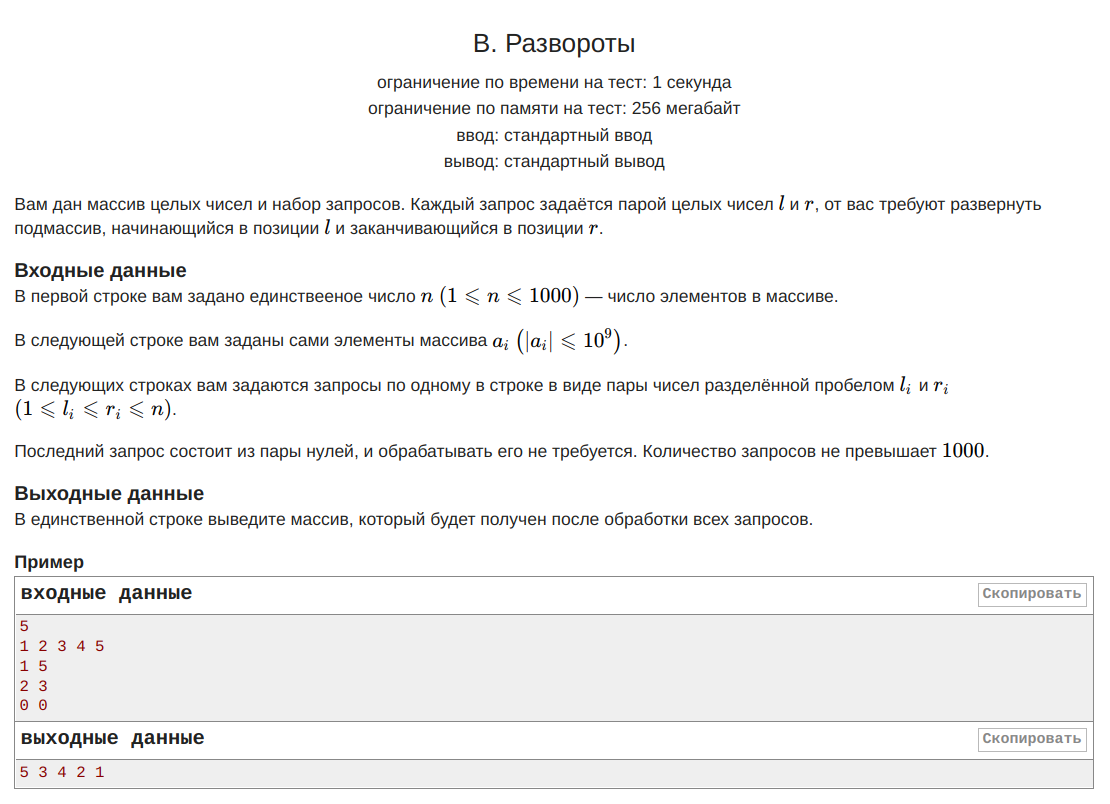
\includegraphics[width=\textwidth]{statements/Contest1B.png}
\end{center}

% Contest-1. Задача B
\subsubsection*{Идея решения}

В первую очередь мы вводим количество элементов в массиве, затем – последовательность в массив, а затем записываем порядки элементов, которые мы поменяем местами.
Далее мы производим операцию swap нужных элементов (не забывая увеличивать индекс начала подполследовательности и уменьшать индекс ее конца). Далее выводим отсортированную последовательность.
Сложность алгоритма $O(m \cdot n)$, где $m$ - количество запросов, а $n$ - длина разворачиваемой подпоследовательности

% {\bfseries \large Например}
% Переборное решение работает $O(n!)$, это очень долго. Использую метод динамического программирования, $dp_i$ --- это минимальное количество белочек при условии чего-то там для $i$ веточек. Это позволяет решить задачу за $O(n ^ 2)$. Дерево отрезков с отложенными обновлениями позволяет улучшить асимптотику до $O(n \cdot \log{n})$, так как все операции с деревом соврешаются за $O(\log{n})$.

\subsubsection*{Исходный код}
% \textit{Исходный код необходимо комментировать, но не более 25\% строк}
\lstinputlisting{src/Contest1B.cpp}

\subsubsection*{Выводы}
Задача решена.
%Задача решена. \textbf{ИЛИ} Задача дорешана. \textbf{ИЛИ} Не принята чекером. Ошибки, неудачи, как они преодолевались.

\newline

\begin{center}
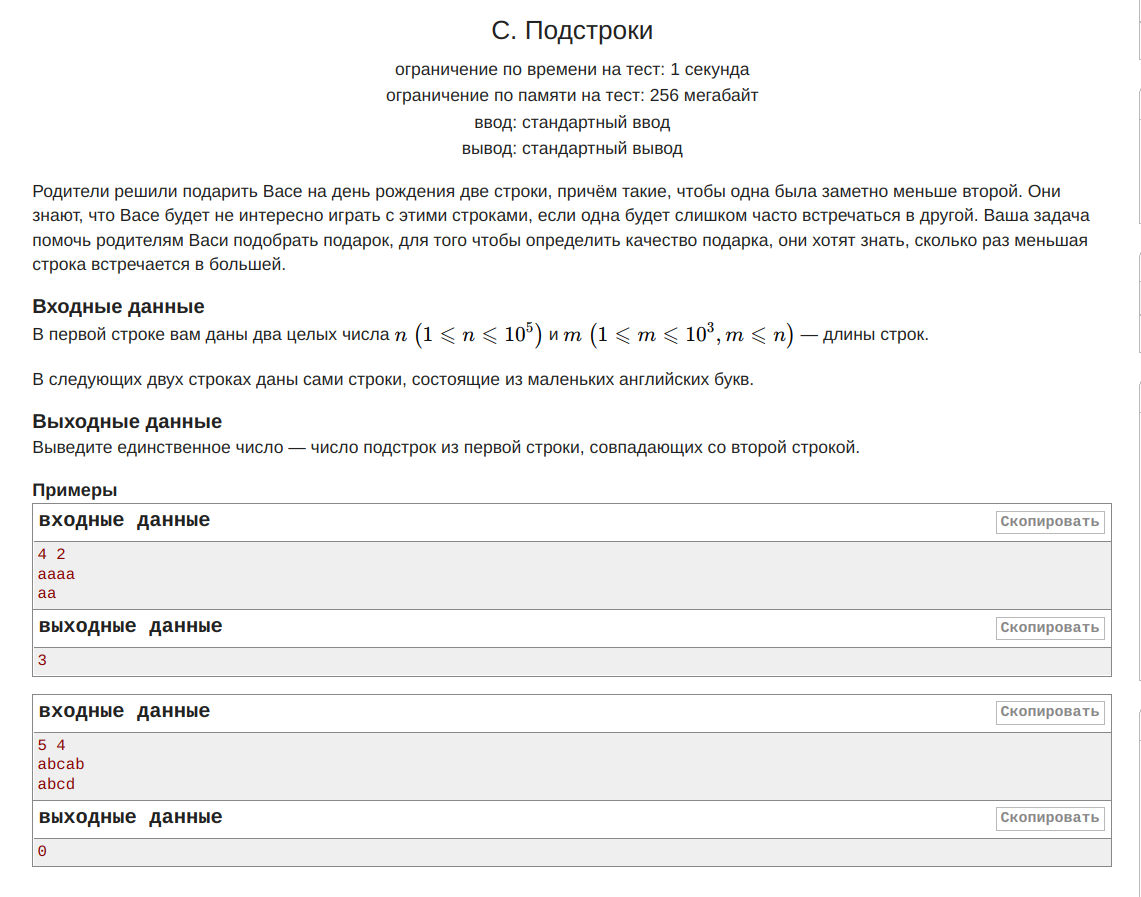
\includegraphics[width=\textwidth]{statements/Contest1C.png}
\end{center}

% Contest-1. Задача C
\subsubsection*{Идея решения}

Для хранения строки и подстроки будеем использовать вектор типа \textit{char}
Далее используем алгоритм прямого поиска подстроки в строке.

\newline

\textbf{Алгоритм прямого поиска подстроки в строке:} 
\begin{enumerate}
    \item i = 1
    \item сравнить i-й символ массива T с первым символом массива W
    \item совпадение → сравнить вторые символы и так далее
    \item несовпадение → i:=i+1 и переход на пункт 2
\end{enumerate}

Сложность алгоритма $O(n \cdot m)$, где $m$ - длина строки, а $n$ - длина подстроки

\subsubsection*{Исходный код}

\lstinputlisting{src/Contest1C.cpp}

\subsubsection*{Выводы}
Задача решена.


\subsubsection*{Фрагмент турнирной таблицы контеста}
\begin{center}
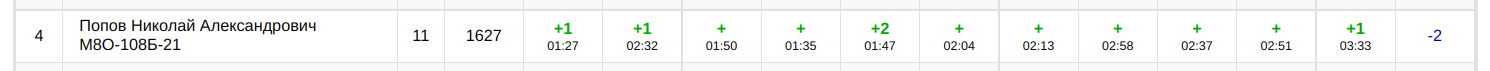
\includegraphics[width=\textwidth]{standings/Contest1Result.png}\newline\noindent
\end{center}


\vspace{16pt}

\pagebreak
